\documentclass[11pt]{report}
\usepackage[utf8]{inputenc}
\usepackage[a4paper, total={6in,8in}, portrait, margin=0.7in]{geometry}
\usepackage{amssymb}
\usepackage{array}
\usepackage{graphicx}
\usepackage{amsmath}
\usepackage{amsfonts}
\usepackage{float}
\usepackage{mathtools}
\usepackage{listings}
\usepackage{xcolor}
\usepackage[misc]{ifsym}
\usepackage{indentfirst} 
\usepackage{amsthm}
\usepackage{appendix}
\usepackage{fancyhdr}
\usepackage{tikz}
\usetikzlibrary{positioning}
\pagestyle{fancy}


%Headers and Footers, thanks to Overleaf
%https://www.overleaf.com/learn/latex/How_to_Write_a_Thesis_in_LaTeX_(Part_2):_Page_Layout
\fancyhead{}
\fancyhead[RO,LE]{\small Improving Duckworth-Lewis: Statistical Methods for Revising Score Targets in Limited-Overs Cricket}
\fancyfoot{}
\fancyfoot[LE,RO]{\thepage}
\fancyfoot[LO,CE]{Chapter \thechapter}
\fancyfoot[CO,RE]{Matthew Knowles}

\DeclarePairedDelimiter{\ceil}{\lceil}{\rceil}

\newtheorem{theorem}{Theorem}[section]
\newtheorem{remark}[theorem]{Remark}
\newtheorem{definition}[theorem]{Definition}
\newtheorem{example}[theorem]{Example}
\newtheorem{lemma}[theorem]{Lemma}

\definecolor{codegreen}{rgb}{0,0.6,0}
\definecolor{codegray}{rgb}{0.5,0.5,0.5}
\definecolor{codepurple}{rgb}{0.58,0,0.82}
\definecolor{backcolour}{rgb}{0.95,0.95,0.92}

\lstdefinestyle{mystyle}{
    backgroundcolor=\color{backcolour},   
    commentstyle=\color{codegreen},
    keywordstyle=\color{magenta},
    numberstyle=\tiny\color{codegray},
    stringstyle=\color{codepurple},
    basicstyle=\ttfamily\footnotesize,
    breakatwhitespace=false,         
    breaklines=true,                 
    captionpos=b,                    
    keepspaces=true,                 
    numbers=left,                    
    numbersep=5pt,                  
    showspaces=false,                
    showstringspaces=false,
    showtabs=false,                  
    tabsize=2
}

\lstset{style=mystyle}

\begin{document}

\begin{titlepage}

    \begin{center}

        \vspace*{1.5cm}

        \textbf{\huge Improving Duckworth-Lewis: Statistical Methods for Revising Score Targets in Limited-Overs Cricket} 
        
        \vspace*{1.5cm}
        
        \textit{Matthew Knowles}

        \vspace*{1.5cm}
    
        
\includegraphics[scale=0.5]{figures/uoylogo.png}
        
        \vspace*{1.5cm}
        
        Department of Mathematics, \\
        University of York, \\
        United Kingdom \\

        \vspace*{1.5cm}

        \textit{A dissertation submitted in partial fulfillment of the requirements for the degree of Master of Mathematics}
    \end{center}
    
\end{titlepage}

\section*{Abstract}
Write this last

%\section*{Acknowledgements}
%The author would like to thank Dr. Jessica Hargreaves for their invaluable supervision and advice throughout this project. Secondly, my eternal thanks and admiration for my friends in York, who have made my time here so wonderful from the very begining, and for all the support you have given me every step of the way. 
%My thanks to Michael Najdan at Kent County Cricket Club for his insight into how data is used in the professional game of cricket.
%Finally, to the UYMCC, who have enriched my university experience beyond belief. 


\section*{Notes}
All code written in support of this project can be found on GitHub at: \\
\textit{https://github.com/mattknowles314/mastersThesis}.

\setcounter{tocdepth}{0}
\tableofcontents

\setcounter{tocdepth}{1}
\listoffigures


\input{Chapters/Intro}

\chapter{Data}

\epigraph{One person's data is another person's noise}{K.C. Cole}

The purpose of this small chapter is to give an overview of the data that is used for this project.

\section{Data Origin}
The primary source of data for carrying out this project was downloaded from ``cricsheet''\footnote{https://cricsheet.org/}
and stored locally on a private server. In total there are 2167 individual matches of data. Each in a JSON format, 
covering matches ranging from the $3^{rd}$ of January 2004 to the $20^{th}$ of July 2021. \\

There is actually an R package, \verb|cricketdata| that allows for the direct import of data from ESPNCricinfo\footnote{https://www.epsncricinfo.com}
and Cricsheet. However this package was published in February 2022, several months after the bulk of work on this project started. In hindsight, using this package 
would have been a lot easier and saved a considerable amount of time. With that in mind, future work on the \verb|CricNet| package (See Appendix C)
will incrorperate this package to streamline the analysis pipeline as a whole. 

\section{Attributes}
Each JSON file contains a considerable amount of metadata surrounding the match in question, along with 
ball-by-ball data for the entire match. We have access to attributes such as the date, where the match was played,
the entire teamsheet for both teams, who the officials were, who won- and by what margin, who won the toss; and many others.

We also have the ball-by-ball data. So for every ball bowled, it gives who were the striking and non-striking batsmen, how many runs
were scored and how. It also details if a wicket was taken that ball, and how.

\section{Pre-Processing}
In order to clean data and make it usable, Python scripts were written to take the original JSON files and turn them into CSV files on which analysis could 
be performed in R. These scripts made heavy use of the base-Python libraries \verb|JSON| and \verb|CSV|.

\section{Problems}
When it comes to machine learning, the more data the better is a general rule. Now this can sometimes lead to sub-problems, such as overfitting. But on the whole 
it is much better to have as much data as possible. We will be training a neural network on 1435 data points. Stictly speaking, this isn't a lot of data, but there
isn't much that can be done about this due to the cricketing calender only having a certain number of limited-overs matches each year.


\chapter{The DLS Method in Detail}

We now look at the mathematics behind the D/L, and DLS methods. D/L being the original
method, and DLS the method that Stern helped to revise. In the original paper, the authors
state ``Commercial confidentiality prevents the disclosure of the mathematical definitions
of these functions.'' $\cite{duckworth}$. Which is naturally a slight problem for this, but what
we can do is instead use sample values based on data we have to look at how these functions behave,
so all is certainly not lost.

\section{Origins: Duckworth and Lewis}
We begin by looking at the original paper. The first thing to establish is how many runs are scored,
on average, in a given number of overs. This is given by the equation:

\begin{equation}
    Z(u) = Z_0[1-exp(-bu)]
    \label{Z(u)}  
\end{equation}

Where u is the number of overs, b is the exponential decay constant, and $Z_0$ is the
average total score in first class cricket, but with one-day rules imposed.  

Now because we don't have access to actual values for $Z_0$ or b, a plot to see what equation \ref{Z(u)} looks 
like was created by using 3 sample values for $Z_0$. For b, it was a process of trial and error to find a value
that resulted in the graph having a similar shape to original figures in the D/L paper. 

\begin{figure}[h]
    \centering
    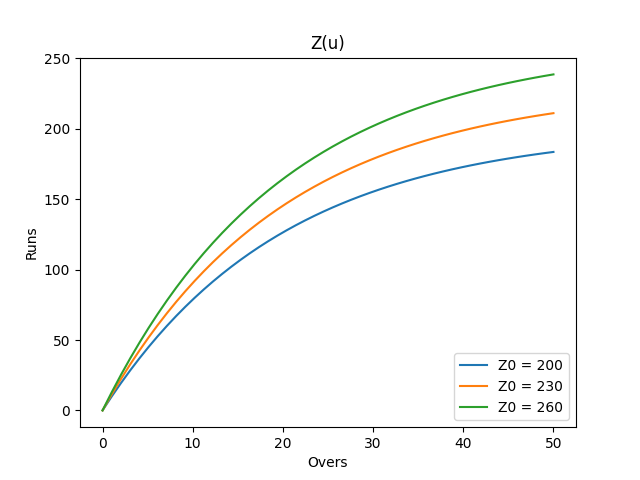
\includegraphics[scale=0.6]{figures/z(u).png}
    \label{Z(u)_graph}
\end{figure}

However, we have not yet looked at what happens when wickets are lost. To introduce this metric, equation \ref{Z(u)}
is revised to incorperate the scenario that w wickets have been lost, and that there are u overs remaining
The revised equation is given as follows:

\begin{equation}
    Z(u,w) = Z_0(w)[1-exp(-b(w)u)]
    \label{zuw}
\end{equation}

Where now, we have $Z_0(w)$ giving the average total score from the last $10-w$ wickets in first class cricket.
We now also have $b(w)$ as the exponential decay constant, which now changes depending on wickets lost.

%Should probably make a plot of this, to go with the other one, but due to confientiality
%it's quite hard to get the numbers for Z0(u,w) myself.

With this in mind, we now look at the specific case of equation \ref{zuw} with $u=N$ and $w=0$, namely, the conditions
at the start of an N-over innings. We have:

\begin{equation}
    Z(N,0) = Z_0[1-exp(-bN)].
    \label{zstart}
\end{equation}

Which we then incorperate into the ratio

\begin{equation}
    P(u,w) = \frac{Z(u,w)}{Z(N,0)}.
    \label{prat}
\end{equation}

The ratio \ref{prat} gives, keeping in mind there are u overs still to be bowled, with w wickets
lost, the average proportion of the runs that still need to be scored in the innings. 
It is this ratio that is where the revised scores come from. Let us now look a bit more at how that works
practically.

\begin{example}
    \label{dlExMain}
    Assume there is a break in the second innings (due to rain or similar), which results in the second team missing some overs.
    Let $u_1, u_2$ be the number of overs played before the break, and available after it respectively. We impose the condition
    that $u_2 < u_1$. At the time of the break, the second team had lost $w$ wickets. The aim is to adjst the required score to account
    for the $u_1 - u_2$ overs they have lost. The winning ``resources'' available are given by

    \[
        R_2 = [1-P(u_1,w)+P(u_2,w)].
    \]  

    Which means, if the first team batting scored S runs, then the new tartget is given by

    \[
        T = \ceil{SR_2}
    \]  
\end{example}

\section{Improvements by Stern}
foo

\chapter{Exploratory Data Analysis}

\epigraph{Cricket often leaves you scratching your head}{James Anderson}

The purpose of this chapter is to explore the obtained dataset in more detail, which is necessary for carrying out the work in later chapters. In general, and no less
in the world of statistics, making assumptions is dangerous, and so in order to make the assumptions we do in later chapters, we must have the evidence to back it up.
This chapter not only provides that evidence, but allows us to become more familiar with our dataset, and see how modern data fits in with the previous work done in this 
field. \\
We begin by looking at the probability densities in the Fall of Wicket variables. F.o.W is key in the DLS method, so we do this to get an idea of what lies underneath the
surface. We are able to explain the way F.o.W distributions are shaped based on the way cricket games unfold. This consistency allows us to make an assumption about Run Rates
later in the chapter too. \\
As with any dataset, there are outliers, and the number of such will have influence on the error function that we use in later models. For that reason, we give brief discussion 
to this, before going on to look at whether or not scores in games of cricket are normally distributed around some mean. \\
Run Rates are the discussed in more detail, looking at whether or not the runrates in certain periods of the game also follow a normal distribution. Finding this out is imperative
for using Monte-Carlo simmulation later on in the paper.

\section{Fall of Wicket Densities}

In this chapter, we are looking only at the first innings of the games, and only those games in which the full 50 overs were played. The 
reason for this is the models we will build are going to try and predict a score as if a full innings has been played. We begin our exploration of the data with a look at how the density of the runs scored per fall of wicket changes. This has been done for each
individual team in the dataset, and in Figures~\ref{ovrdens1fow}-\ref{ovrdens9fow}, we can see how this evolves.  

\begin{figure}
    \centering
    \begin{minipage}{0.4\textwidth}
        \centering
        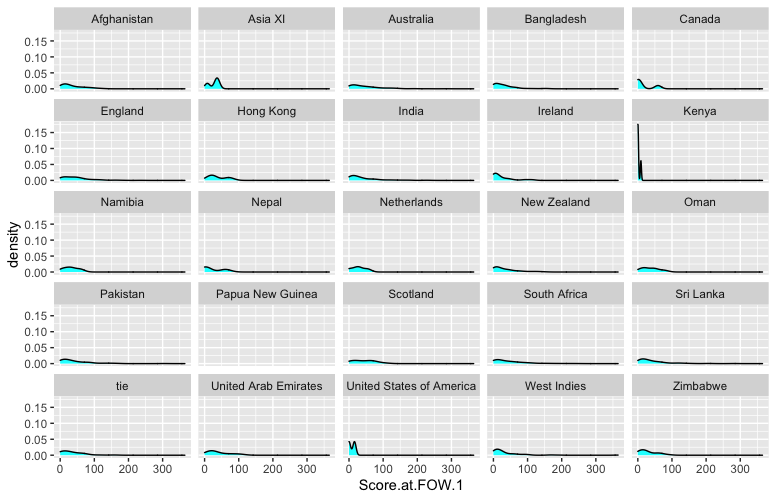
\includegraphics[scale=0.28]{figures/fow1density.png}
        \caption{Density of all teams for first wicket falling}
        \label{alldens1fow}
    \end{minipage}
    \begin{minipage}{0.4\textwidth}
        \centering
        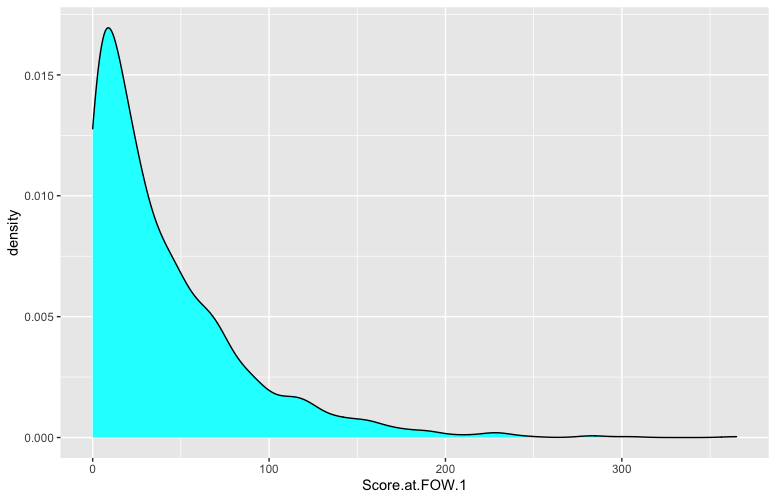
\includegraphics[scale=0.28]{figures/fow1densFull.png}
        \caption{Overall density plot for FOW 1}
        \label{ovrdens1fow}
    \end{minipage}
\end{figure}

\begin{figure}
    \centering
    \begin{minipage}{0.4\textwidth}
        \centering
        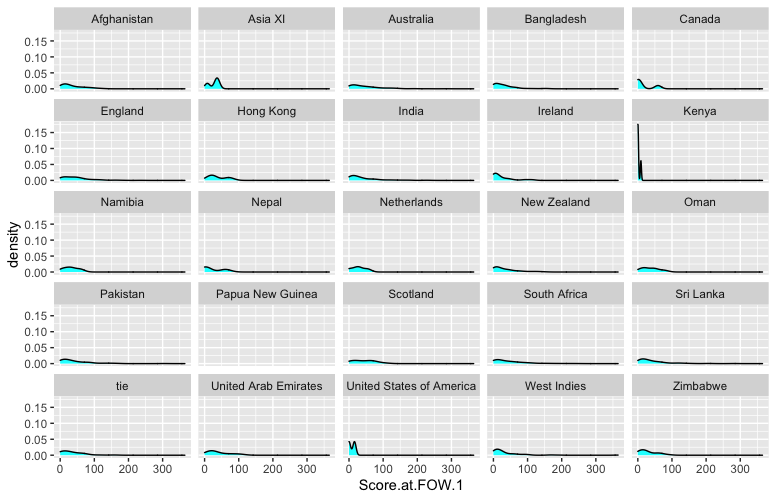
\includegraphics[scale=0.28]{figures/fow1density.png}
        \caption{Density of all teams for fith wicket falling}
        \label{alldens5fow}
    \end{minipage}
    \begin{minipage}{0.4\textwidth}
        \centering
        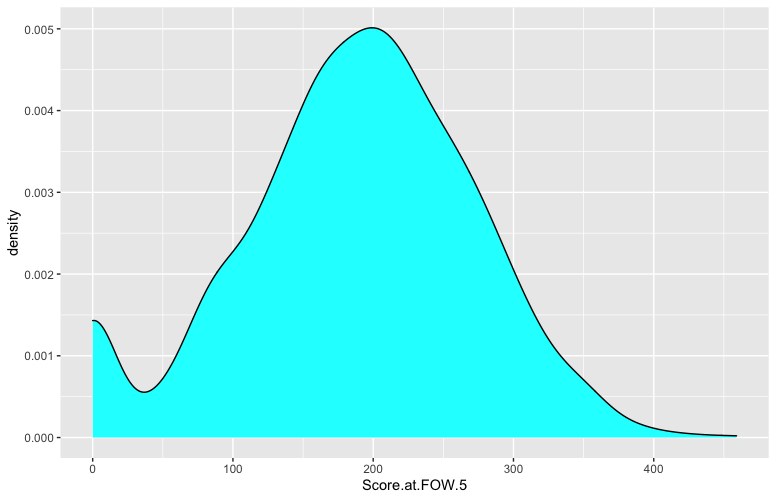
\includegraphics[scale=0.28]{figures/fow5densFull.png}
        \caption{Overall density plot for FOW 5}
        \label{ovrdens5fow}
    \end{minipage}
\end{figure}

\begin{figure}
    \centering
    \begin{minipage}{0.4\textwidth}
        \centering
        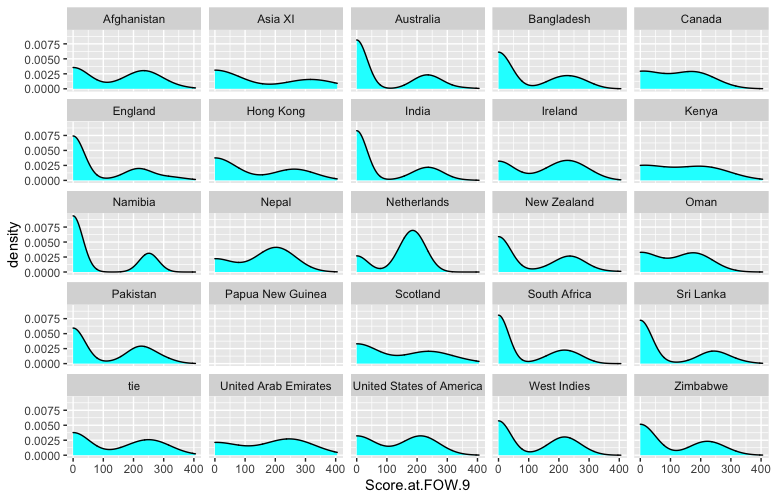
\includegraphics[scale=0.28]{figures/fow9density.png}
        \caption{Density of all teams for ninth wicket falling}
        \label{alldens9fow}
    \end{minipage}
    \begin{minipage}{0.4\textwidth}
        \centering
        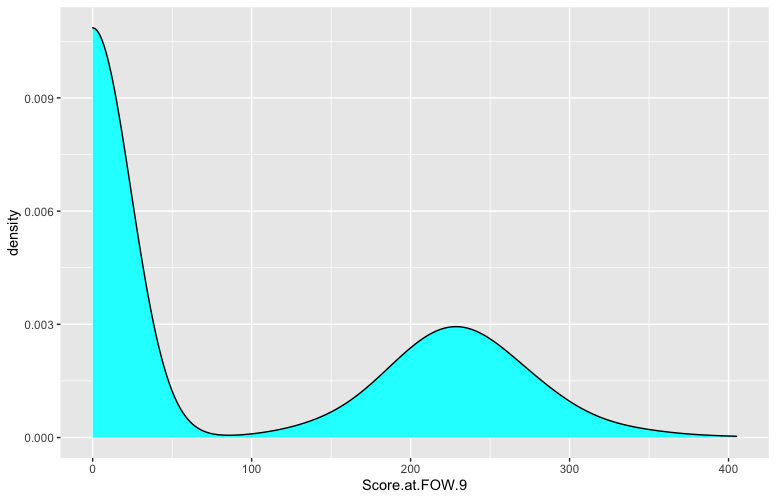
\includegraphics[scale=0.28]{figures/fow9densfull.png}
        \caption{Overall density plot for FOW 9}
        \label{ovrdens9fow}
    \end{minipage}
\end{figure}

In Figure~\ref{ovrdens1fow}, we see the density is heavily skewed to the left. This makes sense, as the bowling team will presumably be starting 
their innings by using their best bowlers, who will be hunting to get wickets early on. In Figure~\ref{ovrdens5fow}, we see a much more normally distributed
density function. But in actual fact, we see this interesting second, smaller peak appearing lower down in the score. Does this make sense? It's certainly 
not suprising. What these two peaks exemplify is the fact games can go heavily in favour of the bowling team, which can be seen in the first small peak,
wherein they have taken a lot of wickets in quick succession, meaning the lower order batters are coming in to bat earlier than usual. Secondly, it shows when the 
batting team is having a good day, because we have this much larger peak around the 200 runs mark.\\

Finally, in Figure~\ref{ovrdens9fow}, we can see that the earlier bowling advantage peak is much higer, because the lower order batters are traditionally less skilled 
at batting, and so the bowling team have a distinct advantage in taking wickets against these players. But we also see the second, batting-favoured peak is no much lower.
This corresponds to the scenario in which the earlier batters have laid a good foundation of the game, and the lower-order batters have not had to contribute much to the score.

\section{Outliers in Runs Data}
\label{mse}
In the next chapter, it will be necessary to choose a loss function for improving the neural network that we create. To aid in determining which function to use, we need to look at the
spread of runs scored in a full innings of data. This can be seen in Figure~\ref{runsbox}.

\begin{figure}[h]
    \centering
    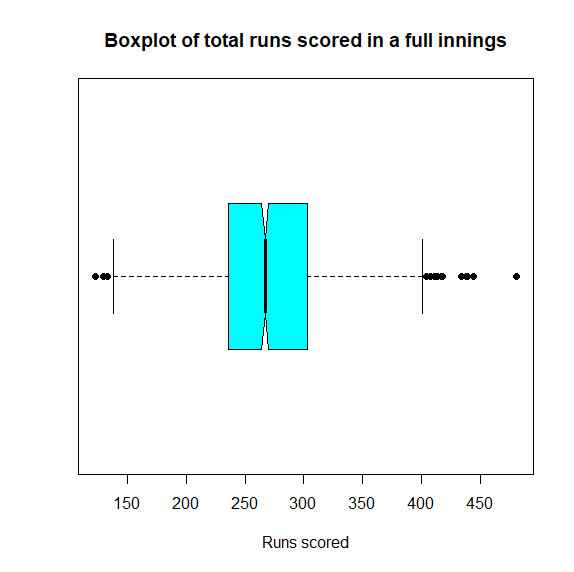
\includegraphics[width=0.4\linewidth]{figures/runsbox.png}
    \caption{Boxplot showing the spread of runs scored}
    \label{runsbox}
\end{figure}

There are 363 data points greater than the third quartile, while 671 are below the first quartile. So $25.3\%$ of our data lies above the third quartile, and
$46.7\%$ below the first. For that reason, we make the decision to use the Mean-Squared-Error (MSE) loss function, which is commonplace in regression problems.

\section{On the Normality of Run Totals}
It will be useful in later parts of this dissertation to know whether or not scores are normally distributed. To test whether or not 
they are, we use a Q-Q plot to check. This is a graphical way for checking normality, by comparing the quantiles of a dataset (in this case, scores) to quantiles
drawn from a theoretical distribution. If the resulting points follow a straight line, it is likely that the data came from the distribution.
In this case, we use the R function \textit{qqnorm()} to test if the runs from the 1436 games of a full 50 overs follow a normal distribution. See Appendix A for 
a more detailed discussion of this method.

\begin{figure}[h]
    \centering
    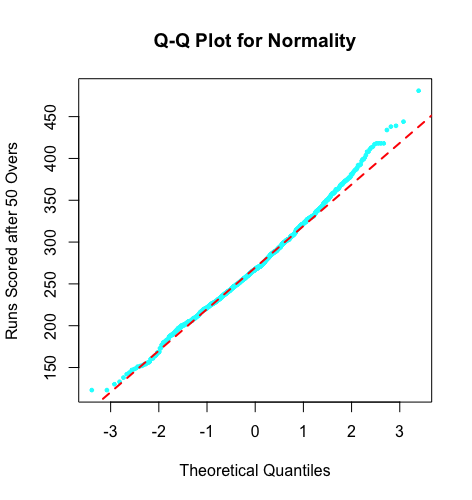
\includegraphics[width=0.4\linewidth]{figures/qqnormplot.png}
    \caption{Q-Q plot for runs scored after 50 overs.}
    \label{qqplot50}
\end{figure}

We can see from Figure~\ref{qqplot50} that the plot follows along the straight line and so we can conclude that the scores are infact normally distributed. 
Further, we can calculate the parameters of this distribution using the R functions \textit{mean()} and \textit{var()}. Doing so gives that the distribution
of scores in 50 overs, $S_{50}$, can be given as $S_{50} \sim \mathcal{N}(270.56,51.34^2)$. \\ 

To further test that this is indeed the case, we can create a sample plot based on this distribution, which can be seen in Figure~\ref{samplenorm}

\begin{figure}[h]
    \centering
    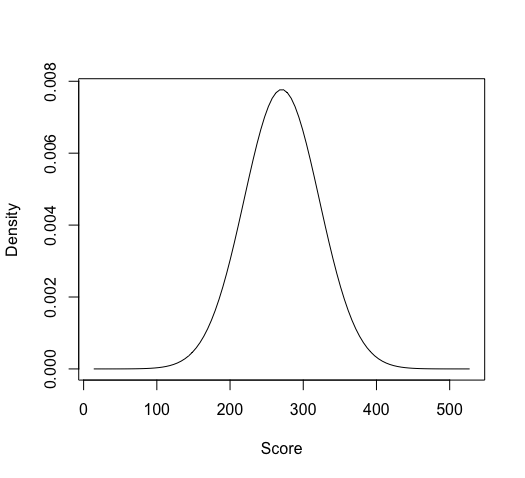
\includegraphics[width=0.4\linewidth]{figures/samplenorm.png}
    \caption{Sample plot created from the derived distribution of $S_{50}$}
    \label{samplenorm}
\end{figure}

With this in mind, we can now look at a density plot for the actual data. This is given in Figure~\ref{errDistAndQQRunsScored}.

\begin{figure}[h]
    \centering
    \subfloat[\centering Density for Runs Scored]{{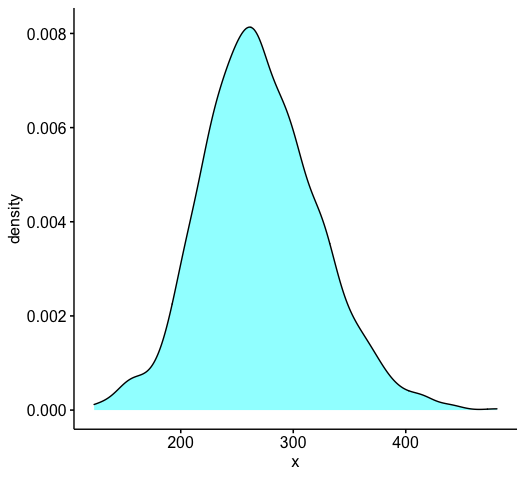
\includegraphics[width=.4\linewidth]{figures/runsdensity.png} }}
    \qquad
    \subfloat[\centering Q-Q Plot for First Innings]{{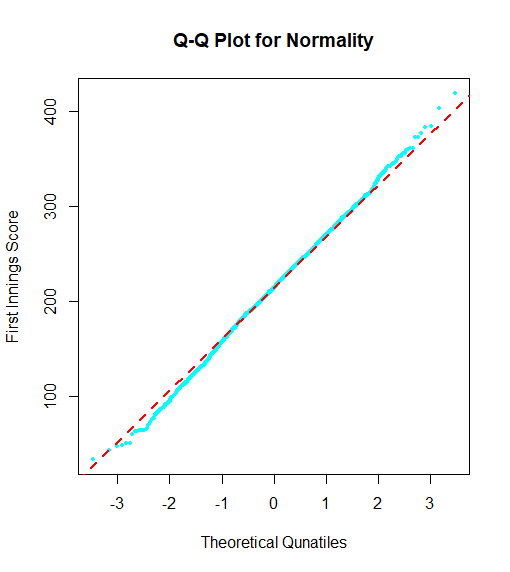
\includegraphics[width=.4\linewidth]{figures/firstInnsQQ.png} }}
    \caption{Error Density and QQ for 50-over Data}
    \label{errDistAndQQRunsScored}
\end{figure}

It is unsuprising that runs are normally distributed, but to be able to draw a mean and variance from this will be very helpful in future aspects of the project.

We have seen that first innings scores in a full 50 overs are normally distributed. We can check, using the same methods if runs in a first innings that 
doesn't necessarily go for the full allowance of overs is normally distributed. 

We find that $S_{FI} \sim \mathcal{N}(213.49,56.91^2)$. 

\section{Run Rates}
\label{exprr}

\subsection{General Exploration}
The work that follows in this section is essential for allowing the Neural Network constructed in Chapter 5 to predict the scores of games. The aim of this section is 
to see if we can draw the run rates at specific overs from a statistical distribution. This will in turn enable us to fill the gaps in the missing overs of a game. In turn, 
with the gaps filled, we can pass the simmulated run rates to the neural network, and allow for a score to be predicted. \\

\begin{figure}[h]
    \centering
    \subfloat[\centering Average run rate per over]{{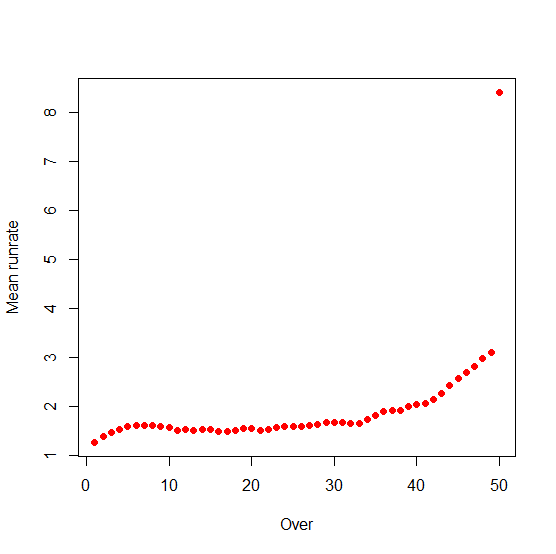
\includegraphics[width=.4\linewidth]{figures/avgRR.png} }}
    \qquad
    \subfloat[\centering Run rate Standard deviation per over]{{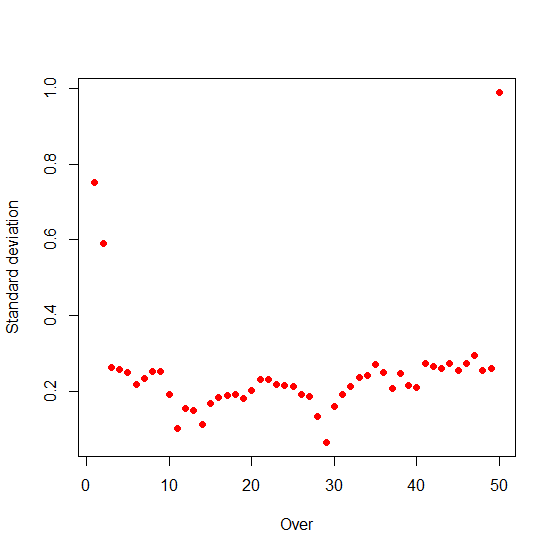
\includegraphics[width=.4\linewidth]{figures/sdrr.png} }}
    \caption{Error distribution with Q-Q plot}
    \label{errDistQQ3}
\end{figure}
\label{errdistqq3}
We can see from Figure~\ref{errDistQQ3}, that average Run Rate seems to stay consistent in the middle overs, before rapidly increasing as the risk associated with losing 
a wicket falls off due to the end of the innings coming closer. If we break the game into five ten-over segments, as these are generally different periods of the game
from a tactical perspective\footnote{This is to do with different bowling options being used to be more effective as the pitch conditions change}, we can model the segments.
A game of ODI-cricket can roughly be broken up to three segments, the first 10 overs, known as the ``powerplay'', where teams are slightly more conservative and look to build a 
foundation on which the rest of the game is built. The middle overs are 11-35. The idea of this game is to continue building on the foundation, and save wickets. The last 
15 overs are where more risks are taken, as the value of a wicket decreases. The rule of thumb for the batting team is to double your score from the first 35 in the last 15, which is why we see the massive 
increase in run rate in these last overs. \\

Using this information, we can create density plots of the average Run Rate in these overs, as in figures 4.13-4.15. 

\begin{figure}
    \minipage{0.32\textwidth}
      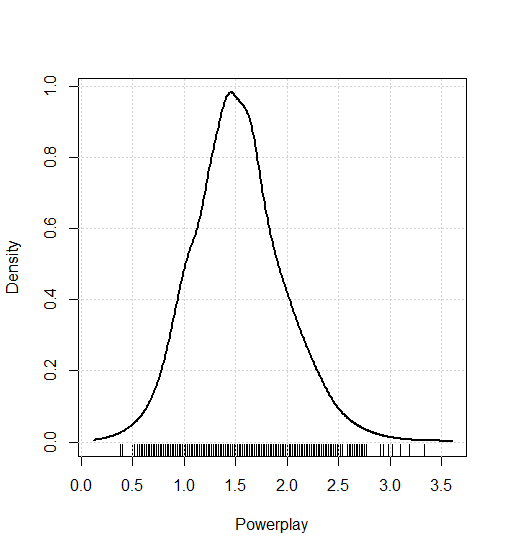
\includegraphics[width=\linewidth]{figures/powerplaydens.png}
      \caption{Powerplay Run Rate density}
    \endminipage\hfill
    \minipage{0.32\textwidth}
      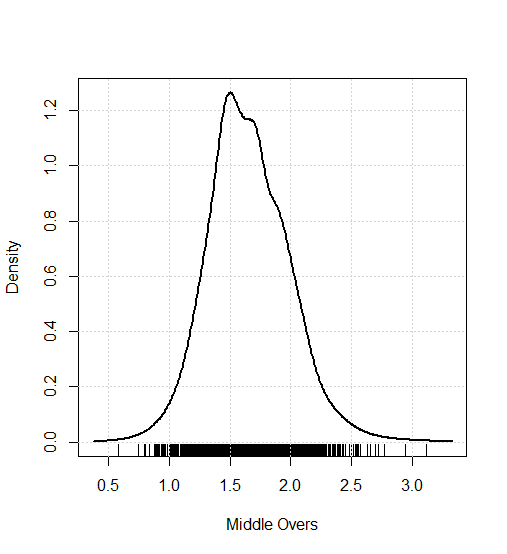
\includegraphics[width=\linewidth]{figures/middleoversdens.png}
      \caption{Middle Overs Run Rate density}
    \endminipage\hfill
    \minipage{0.32\textwidth}%
      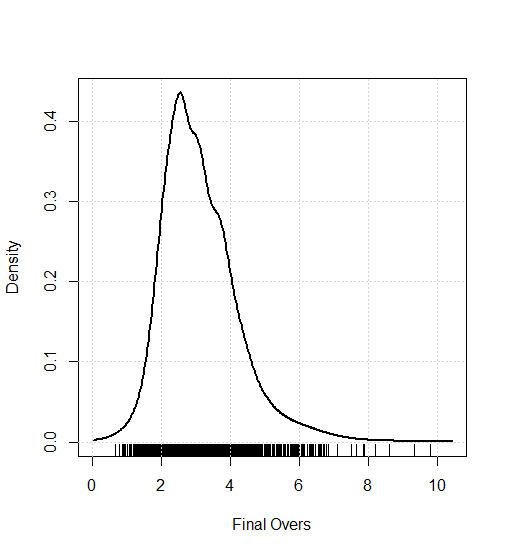
\includegraphics[width=\linewidth]{figures/finaloversdens.png}
      \caption{Final Overs density}
    \endminipage
    \label{rrDensitiesPlot}
\end{figure}

The run rates are  in different stages of the game roughly normally distributed, which can be seen in Figure~\ref{rrDensitiesPlot}. It is reasonable that due to the Central Limit Theorem, with more observations, these distribiutions would be smoothed out and 
appear more normally distributed than it does at present. This is imporant, because it allows us to investigate using a monte-carlo method to fill in gaps 
later on in the project.

\subsection{Feature Selection}
\label{lassoSec}

Feature selection is an important aspect in data science. Some experiments can have an overwhelming number of variables, which can lead to computational inefficiency. In this subsection, we will explore selecting the most important overs in the run rate data.
Given the lack of data already available, this may seem unnecessary, however it is an interesting consideration for future work. When we build the network in the next chapter, the model has to be passed a formula, telling it how to treat the variables. By default, since we have 50 overs worth of data (V1 $\rightarrow$ V50) and a variable containing the final score, V51, we pass the R formula $V51 ~ V1 + \ldots + V50$. The purpose of this section is to see if it is worth reducing this somewhat combersome formula. 
LASSO, \textbf{L}east \textbf{A}bsolute \textbf{S}hrinkage and \textbf{S}election \textbf{O}perator, is a regression method for performing both normalisation, and feature selection. The term LASSO was introduced by \cite{tib}. Before showing how we implement this in R, and what it means for our project, it is useful to discuss the mathematical foundation of the method, as in section 2.1 of Tibshirani's paper. \\

For $i=1,\ldots,N$, we have a dataset $(\textbf{X}^i,y_i)$. For the training dataset we use, $N=1436$. Specifically, we define $\textbf{X}^i = (x_{i1},\ldots,x_{ip})$ to be the vector of predictor variables (for us, $p=50$). Further, $y_i$ is the response variable. The assumption that these variables are independent is immediately satistfied by the nature of our study, since the runs scored in one over does not depend at all on the runs scored in the prior over. In addition, our data is normalised when it is passed the neural network, and so the normalisation assumption is also satistfied by default. 

\begin{definition}
    We begin by letting $\beta = (\hat{\beta_1},\ldots,\hat{\beta_p})^T$, then the \textbf{LASSO estimate} $(\hat{\alpha}, \hat{\beta})$, for a tuning parameter $t \geq 0$ is given by
    \[
        (\hat{\alpha},\hat{\beta}) = \text{argmin} \left\{ \sum_{i=1}^N \left(y_i - \alpha - \sum_j \beta_j x_{ij} \right)^2 \right\} \\
    \]
    Suject to $\sum_j |\beta_j| \leq t$. 
\end{definition}

We have that $\forall t$, $\hat{a} = \bar{y}$. However since the data is normalised, by defintion $\bar{y}=0$ and so we can ignore the parameter $\alpha$ altogether. Although not discussed directly here, the authors do go on to propose algorithms for computing solutions to this problem in chapter 6 of their paper. These algorithms are employed directly by the R package \verb|glmnet|, which we can now use. \\

We use the function \textit{cv.glmnet()}. This can be seen in the following code snippet.

\begin{figure}[h]
    \lstinputlisting[language=R, firstline=6, lastline=7]{../Code/Rscripts/lasso.R}
    \caption{Fitting a LASSO model}
    \label{lassoCode}
\end{figure}

The plot produced by this code can be seen in Figure~\ref{lassoFig}.

\begin{figure}[h]
    \centering
    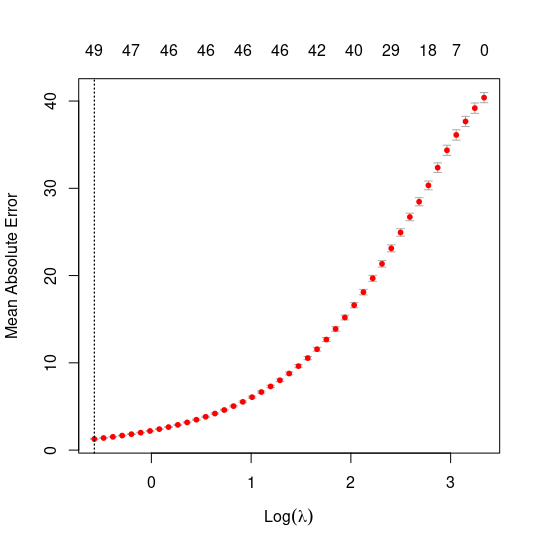
\includegraphics[width=0.5\linewidth]{figures/lasso.png}
    \caption{LASSO Model Plot}
    \label{lassoFig}
\end{figure}

The red dots here show the mean absolute error when the number of variables used in the model. We can see from this plot that using all of the overs results in the lowest MAE. Seeing which variables contribute the most can be done using the code in Figure~\ref{lassoVals}. 

\begin{figure}[h]
    \lstinputlisting[language=R, firstline=12, lastline=13]{../Code/Rscripts/lasso.R}
    \caption{Contributing Variables}
    \label{lassoVals}
\end{figure}

This code orders the variables depending on how ``important'' they are. This ordering is done by the minimum lambda value. As it turns out, the 5 most important overs are 31, 46, 35, 38 and 48. Unsuprisingly, the least important is over 1. This is more than understandable from a cricketing standpoint, since a lot can change after the first over, whereas the later overs can make or break an innings. 



\chapter{Pattern Recognition with Neural Networks: Background and Implementation}

\epigraph{Nowadays, with technology coming into cricket, people start to analyse, and if you only have one or two tricks, people will start to line you up}{Jasprit Bumrah}

We begin this chapter by looking at the mathematical background of neural networks. More specifically, the construction of them using Linear Algebra, and then algorithms 
for training them. By ``training'', we mean updating the parameters associated with the network in order to improve their predictive accuracy. After this mathematical discussion, 
we look at using the \verb|neuralnet| package in R to implement a network, although the resulting network is dicussed in the next chapter. The chapter finishes with a discussion of 
time complexity of the algorithms used.

%Explain which langauges were chosen for each method and why

\section{A Brief Introduction to Neural Networks}
Neural networks (NNs) have been the subject to a lot of discussion and exploration in recent years. They are a machine learning method that is being applied to many problems
in all sorts of fields, such as finance \cite{nnstock} and medicine \cite{nncancer}.  
The network will be trained on run rate data, so for each game we have calculated the evolution of the run rate,
and then we have the overall score for that game in the final column of the matrix. An example of a network can be seen in Figure~\ref{nnexample1}. The first layer is the 
input layer, and the last layer gives the predictions. The middle layers are hidden and where the work of the network is done. \\

\begin{figure}
    \centering
    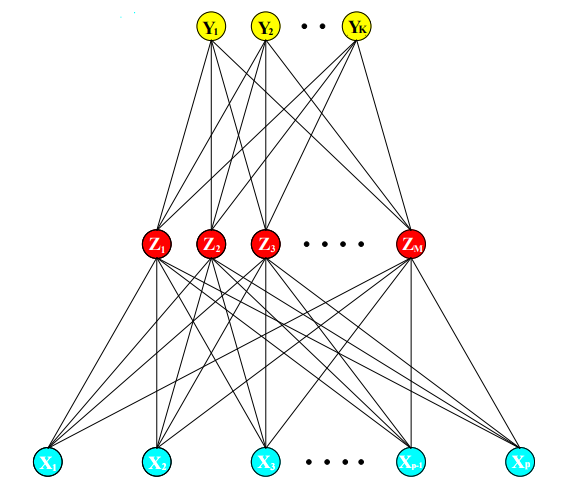
\includegraphics[scale=0.5]{figures/nn.png}
    \caption{Example of a single hidden layer neural network, as in \cite{sprbk}. Inputs are inputted through the bottom layer, the final activity value in the top
    layers are taken as the prediction.}
    \label{nnexample1}
\end{figure}

We see there are $p$ input nodes at the bottom, M nodes in the hidden layer, and K output layers. The lines between the layers are given a ``weight''
and a ``bias''. These properties will be discussed in more detail shortly. The number of hidden layers to be used will be the subject of experimentation. 
It's important to note how we will measure the success of the model. The main dataset, consisting of 1438 games of 50 overs is split into two subsets, one 
containing 70\% of the games, and one containing 30\%. We use the larger of the two to ``train'' the model, and the smaller one as a test set. Not doing this could 
lead to a phenomenom known as ``overfitting''; where the network learns how to predict patterns in the dataset it was trained on really well, but then isn't so good 
at predicting unseen values. We use correlation as the main metric of success in this model, which will be discussed later on.

As mentioned, NNs have been used extensively in finance- more specifically, in predicting future stock price behaviour. Naturally if one can predict how the value of a stock
will change over some time period, then one can protect themselfes from a bad investment, or profit heavily from a good one. We will use similar
methods here for building our neural network.  In \cite{nnstock}, the authors test two different Neural Networks, and find that using a ``Multi-Layer Feed Forward Nerual Network''
is the better choice for predicting how stock values will change. With these motivations in mind, we can begin to construct the networks.

\section{Building The Network}
Our input layer will have 50 nodes, one for the run rate at the end of each over. We will begin with 5 hidden layers, although this is subject to change. The output layer
will of course only have one node, the value of which will predict the score of the game. There will be three hidden layers, with 25, 10 and 3 nodes respectively. 
The ideas is that the prediction is refined over time down to a single value. In the future, more work is needed to experiment with different hidden layer topologies. 

We begin by looking at a single node. The proper name for each node is ``perceptron''. Each perceptron takes in the values of a vector, and an extra ``+1'' intercept term. The perceptron then outputs a value $h$ given by Equation~\ref{percepout}:

\begin{equation}
    \label{percepout}
    h_{W,b}(x) = f(\textbf{W}^Tx) = f(\sum_{i=1}^KW_ix_i+b).
\end{equation}

Here, $K \in \mathbb{N}$ is the number of elements in the vector, and $f:\mathbb{R} \rightarrow \mathbb{R}$ is called the activation function. There is a bit of choice in which activation function to use.
The two common choices are the Sigmoid function (Equation~\ref{sigmoid_func}) and the Hyperbolic Tangent Function:

\begin{align}
    \label{sigmoid_func}
    f(z) &= \frac{1}{1+exp(-z)} \\
    f(z) &= tanh(z)
\end{align}

The comparison of these two functions can be seen in Figure~\ref{actfig}.

\begin{figure}[h]
    \centering
    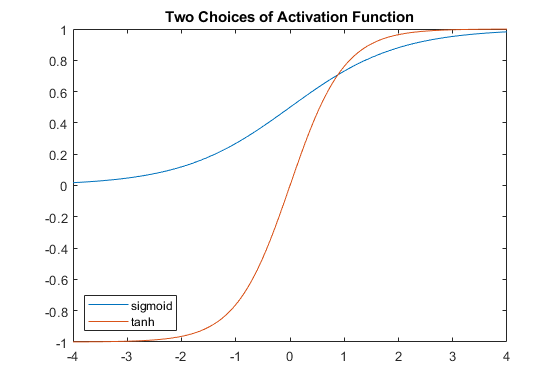
\includegraphics[scale=0.5]{figures/actfuncs.png}
    \caption{Graph showing the shape of different activation functions.}
    \label{actfig}
\end{figure}

We will be using Equation~\ref{sigmoid_func} as our activation function. There is some leniency over which activation function is used. The paper \cite{sibi} found that actually the more important aspect of 
the network is the choice of training algorithm, along with other parameters such as learning rate $\alpha$. For now, lets look at the network we're going to use. 

We begin with getting from the input layer, denoted $L_0$. Each node in $L_0$ takes a value $a^{(0)_i}$ for $i \in \{1,2,\ldots,50\}$. We use $\textbf{a}^{(0)}$ to denote the vector
containing these values. For every node in $L_0$, we have 25 connections coming away, one going to each of the nodes in $L_1$. 25 was an arbitrary choice for the size of $L_1$, and is
subject to change based on results from initial testing. So that means we have $50 \times 25 = 1250$ weights for just the first layer alone. Some linear algebra is to be done here to get 
values for the vector $\textbf{a}^{(1)}$. We use $w_{ij}$ to denote the weight from node j in one layer to node i in the prior layer. We can then construct a matrix containing the weights
between $L_0$ and $L_1$, which we denote $W^{(1)}$. This matrix is given by Equation~\ref{weights1}.

\begin{equation}
    W^{(1)} =
    \left[ {\begin{array}{cccc}
      w_{1,1} & w_{1,2} & \cdots & a_{1,50}\\
      w_{2,1} & w_{2,2} & \cdots & a_{2n}\\
      \vdots & \vdots & \ddots & \vdots\\
      w_{25,1} & a_{25,2} & \cdots & a_{25,50}\\
    \end{array} } \right]
    \label{weights1}
\end{equation}

Using Equation~\ref{weights1}, and combining with $a^{(0)}$, we can get the following:

\begin{align}
    A^{(1)} &= \left[ {\begin{array}{cccc}
        w_{1,1} & w_{1,2} & \cdots & a_{1,50}\\
        w_{2,1} & w_{2,2} & \cdots & a_{2n}\\
        \vdots & \vdots & \ddots & \vdots\\
        w_{25,1} & a_{25,2} & \cdots & a_{25,50}\\
      \end{array} } \right] \times \left[ \begin{array}{c}
          a^{(0)}_1 \\
          a^{(0)}_2 \\
          \vdots \\
          a^{(0)}_{50} \\
      \end{array} \right] + \left[ \begin{array}{c}
        b^{(0)}_1 \\
        b^{(0)}_2 \\
        \vdots \\
        b^{(0)}_{25} \\
        \end{array} \right] \\
      &= W^{(1)}\textbf{a}^{0} + \textbf{b}^1
\end{align}

Where $\textbf{b}^1$ is the vector containing the biases for each node.  At this point, we are incredibly close to having values for $\textbf{a}^{(1)}$. The last thing to do
is apply the activation function. The above has resulted in a $25\times 1$ vector, we use the notation $f(A^{(1)})$ to denote applying the activation function to each 
element in the vector $A^{(1)}$. Putting this all together, we have the following equation:

\begin{equation}
    \textbf{a}^{(1)} = f(W^{(1)}\textbf{a}^{(0)} + \textbf{b}^{1})
\end{equation}

Which gives us values for all the nodes in the first hidden layer. This process is then repeated for each layer, creating a diffferent weights and bias matrix going between each layer in the network. 
These matrices are naturally of different sizes, but the principle is exactly the same. When we start the training process for this network, we will only have random variables for the weights and biases. 
To gain better values that can predict accurate results in the future, we need to train the network by feeding it feature vectors and their associated outputs. \\

To allow the network to be trained, we first must define a ``cost function''. The way we do this is to input a vector to the input layer, let the network produce a result, say $y'$, which
initially is likely to be quite wrong, and square the difference between this and the true value $y$ for that particular training vector. Put more precisely,
let \textbf{X} be a feature vector containing 50 elements, and $y$ the corresponding output. Then define the cost function, $C(X,y) := (y'-y)^2$. The lower the value of $C(X,y)$, the 
better the network has done at predicting. The average value of $C(X,y)$ for each X and y in our training set, is then a good measure of the network's performance. \\

The cost function is at the heart of how these networks ``learn''. All we're doing is minimising a cost function, to give matrices of weights and biases that
produce the best output. The algorithm for minimising this cost function is called ``gradient descent'' \cite{cauchy}.

\begin{example}
    In this example, we initialise four random weights matrices, four bias vectors, and we run through the process outlined above. We know going into this that 
    the cost is going to be high since no learning has been done. Initialising the weights as random values $w_{ij} \in [-1000,1000]$, we get an initial cost function for our full dataset of 
    3098.4. 
\end{example}

\subsection{Training the Network: Gradient-Descent and backpropagation}

We discussed in section \ref{mse} the need to use a MSE loss function based on our data. Let us now define this function, as in \cite{huber}.

\begin{definition}
    Let N be the number of datapoints, $y_i'$ be the predicted value from the $i^{th}$ datapoint, and $y_i$ be the true value. Then for the input vector X, and a parameter $\theta$,
    define the \textbf{Mean Square Error} by
    \begin{equation}
        E(X,\theta) = \frac{1}{2N}\sum^N_{i=1}(y_i'-y_i)^2
    \end{equation}
\end{definition}

The method of \textit{Gradient Descent} necessitates calculating the gradient of $E(X,\theta)$ with respect to weights and biases in each layer. The idea is to find a local minimum, as this will
give a set of weights and biases for which the error is lowest, and such that the network is giving well approximated results. Define a \textit{learning rate} $\alpha$, and incorporate the set of weights
and biases into the parameter $\theta$. Then we update the weights and biases each iteration t via the relationship \ref{graddesc}

\begin{equation}
    \label{graddesc}
    \theta^{t+1} = \theta^t - \alpha\frac{\partial E(X,\theta)}{\partial \theta}.
\end{equation}

With this in mind, we can now start to go through the Backpropagation process. Firstly, we need to calculate the partial differential of E with respect to a given weight $w^k_{ij}$. This calculation is given as follows:

\begin{align}
    \frac{\partial E(X,\theta)}{\partial w_{ij}^k} &= \frac{1}{2N}\sum_{d=1}^N\frac{\partial (y'_d-y_d)^2}{\partial w_{ij}^k} \\
                                                   &= \frac{1}{N}\sum^N_{d=1} \frac{\partial E_d(X,\theta)}{\partial w_{ij}^k}.
\end{align}

In the above, we have $E_d = \frac{1}{2}(y'_d-y_d)^2$.  We must emply the chain rule to calculate the partial derivavtive of $E_d$ with respect to an individual weight. 
Let $a_j^k$ be the activation value of node j in layer k before it is put through the activation function. Then we have

\begin{equation}
    \label{errorchain}
    \frac{\partial E}{\partial w_{ij}^k} = \frac{\partial E}{\partial a_j^k}\frac{\partial a_j^k}{\partial w_{ij}^k}.
\end{equation}

In Equation~\ref{errorchain}, the first derivative on the righthand side, is known as the \textit{error}, often denoted as $\delta_j^k$. The second derivative on that side
is the \textit{output} of node i in layer $k-1$, denoted $o_i^{k-1}$. So we can simplify \ref{errorchain} to be written as

\begin{equation}
    \frac{\partial E}{\partial w_{ij}^k} = \delta^k_jo_i^{k-1}.
\end{equation}

The aim of backpropagation is to minimise the error $\delta^m_1$, where m denotes the final layer. We can express $E_d$ in terms of $a_1^m$ as follows:

\begin{equation}
    E_d = \frac{1}{2} (f(a_1^m)-y_d)^2.
\end{equation}

Where $f$ is the activation function. We have:

\begin{equation}
    \delta_1^m = (y'-y)f'(a_1^m).
\end{equation}

So in the final layer, we have:

\begin{align}
    \frac{\partial E_d}{\partial w_{i1}^m} &= \delta_1^mo_i^{m-1} \\
                                           &= (y_d'-y_d)f'(a_1^m)o_i^{m-1}.
\end{align}

The above works well for the final layer, but we now must consider the hidden layers. We will consider the general case here, and then plug in the relevant
numbers for our model when it comes to the implementation later on. For a layer k such that $1 \leq k < m$, the error term $\delta^k_j$ is given by:

\begin{align}
    \delta_j^k &= \frac{\partial E_d}{\partial a_j^k} \\
               &= \sum_{l=1}^{r^{k+1}} \frac{\partial E_d}{\partial a_l^{k+1}}\frac{\partial a_l^{k+1}}{\partial a_j^k}.
\end{align}

In the above, $r^{k+1}$ is the number of nodes in the next layer, and $ l = 1,2,\ldots,r^{k+1}$. Since we can write $\delta_l^{k+1} = \frac{\partial E_d}{\partial a_l^{k+1}}$, the above can be written
as 

\begin{equation}
    \label{deltajk}
    \delta_j^k = \sum_{l=1}^{r^{k+1}}\delta_l^{k+1}\frac{\partial a_l^{k+1}}{\partial a_j^k}.
\end{equation}

Since the activation of a layer in one node is the sum of weights and avtications in the prior layer, we write:

\begin{equation}
    a_l^{k+1} = \sum^{r^k}_{j=1} w_{jl}^{k+1}f(a_j^k).
\end{equation}

Therefore,

\begin{equation}
    \frac{\partial a_l^{k+1}}{\partial a_j^k} = w_{jl}^{k+1}f'(a_j^k).
\end{equation}

Plugging the above into Equation~\ref{deltajk}, we obtain the following:

\begin{equation}
    \label{backpropform}
    \delta_j^k = f'(a_j^k)\sum^{r^{k+1}}_{l=1}w_{jl}^{k+1}\delta_l^{k+1}.
\end{equation}

The Equation~\ref{backpropform} is known as the \textit{backpropagation formula}. The final step is to calculate, $\frac{\partial E_d}{\partial w_{ij}^k}$, which is given by:

\begin{align}
        \frac{\partial E}{\partial w_{ij}^k} &= \delta^k_jo_i^{k-1} \\
        &=f'(a_j^k)o^{k-1}_i \sum^{r^{k+1}}_{l=1}w_{jl}^{k+1}\delta_l^{k+1}.
\end{align}

\subsection{RPROP+}
Backpropagation is a powerful and widely used algorithm, In implementing the neural network in this project, we used a variation of it, known as 
the ``RPROP+'' algorithm \newline 
\cite{rprop}, short for ``\textbf{R}esiliant back\textbf{PROP}agation''. The $+$ is notation for showing we include backtracking in the algorithm. In Algorithm~\ref{RPROPC}, 
we give the algorithm in detail. 

\begin{algorithm}[h]
    \caption{RPROP+}\label{RPROPC}
\begin{algorithmic}[1]
\ForAll{eights and biases}
\If{$\frac{\partial E}{\partial w_{ij}}(t-1)\times\frac{\partial E}{\partial w_{ij}}(t) > 0$}
    \State $\Delta_{ij} = \text{min} (\Delta_{ij}(t-1)\times \eta^{+},\Delta_{\text{max}})$ 
    \State $\Delta w_{ij}(t) = -\text{sign}\left(\frac{\partial E}{\partial w_{ij}}(t) \times \Delta_{ij}(t)\right)$
    \State $w_{ij}(t+1) = w_{ij}(t) + \Delta w_{ij}(t)$
\ElsIf{$\frac{\partial E}{\partial w_{ij}}(t-1)\times\frac{\partial E}{\partial w_{ij}}(t) < 0$}
    \State $\Delta_{ij} = \text{min} (\Delta_{ij}(t-1)\times \eta^{-},\Delta_{\text{min}})$ 
    \State $w_{ij}(t+1) = w_{ij}(t) - \Delta w_{ij}(t-1)$
    \State $\frac{\partial E}{\partial w_{ij}}(t) = 0 $
\ElsIf{$\frac{\partial E}{\partial w_{ij}}(t-1)\times\frac{\partial E}{\partial w_{ij}}(t) = 0$}
    \State $\Delta w_{ij}(t) = -\text{sign}\left(\frac{\partial E}{\partial w_{ij}}(t) \times \Delta_{ij}(t)\right)$
    \State $w_{ij}(t+1) = w_{ij}(t) + \Delta w_{ij}(t)$
\EndIf
\EndFor
\end{algorithmic}   
\end{algorithm}

What makes RPROP ``resiliant'' is the introduction of an individual update value $\Delta_{ij}$ for each weight $w_{ij}$. It is this quantity alone that determines 
how much the weight will be updated by. The learning rule is given by 

\begin{equation}
    \Delta_{ij}^{(t)} = 
    \begin{cases}
        \eta^{+}\times \Delta_{ij}^{(t-1)} & \text{if} \  \frac{\partial E}{\partial w_{ij}}(t-1)\times\frac{\partial E}{\partial w_{ij}}(t) > 0 \\
        \eta^{-}\times \Delta_{ij}^{(t-1)} & \text{if} \  \frac{\partial E}{\partial w_{ij}}(t-1)\times\frac{\partial E}{\partial w_{ij}}(t) < 0 \\
        \Delta_{ij}^{(t-1)} & \text{otherwise}
    \end{cases}
\end{equation}

As mentioned previously, the $+$ refers to having backtracking in the algorithm. It is helpful to formally define this.

\begin{definition}
    Suppose the partial derivative $\frac{\partial E}{\partial w_{ij}}$ changes sign. This means the prior step was too large, meaning the minimum is missed. For that reason, 
    we \textbf{backtrack} to the previous weight update. I.e,
    \[
        \Delta w_{ij}^k = -\Delta w_{ij}^{(k-1)} \  \text{if} \  \frac{\partial E^{(k-1)}}{\partial w_{ij}} \times \frac{\partial E^k}{\partial w_{ij}} < 0 
    \]
\end{definition}

\section{Implementing the Neural Netowk}
It was decided to implement the neural network using the R programming language, and more specifically, the \verb|neuralnet| package by \cite{gunther}. This package 
allows us to specify all the parameters we wish for, and automatically performs the backpropagation algorithm to train a network. The whole aspect of this process is the encapsulated in line 4
of Figure~\ref{nnRcode}. It was decided to use a prebuilt package for this rather than building it our self since the code for this package has already been optimised, and so will be more efficient 
than an implementation we come up with. Since we would have to take time out to optimise the code and this would detract from the purpose of this project. \\  

Recall the logistic function, $\sigma : \mathbb{R} \to (0,1)$, defined by:
\[
    \sigma(x) = \frac{1}{1+exp(-x)}.
\]

For extremely positive or negative values of $x$, $\sigma$ will return $-1$ or $1$, so we must normalise the data before training the neural 
network. Once the data were normalised, several versions of the network were ran with varying parameters. The final parameters decided were a learning rate, $\alpha = 0.02$, and a hidden network of layers consitsting of 
25 neurons, two layers of 10 neurons, and a final hidden layer of 3 neurons. In total, we ran 1000 iterations, each randomly initialising neuron values by drawing from the $N(0,1)$ distribution. 
The code for this can be seen in Figure~\ref{nnRcode}.

\begin{figure}[h] %MAKE SURE THESE ARE THE RIGHT LINES OF CODE!!
    \lstinputlisting[language=R, firstline=29,lastline=35]{../Code/Rscripts/scoreNet.R}
    \caption{R code to implement the neural network}
    \label{nnRcode}
\end{figure}

A plot of this network can be seen in Figure~\ref{bestnet}. Implementing the network this way is fairly efficient, and does not cause any issues with time-complexity. Infact, backpropagation 
was found to have a median time complexity of $\mathcal{O}(N^4)$ in \cite{lister}. Running 1000 training iterations took ~10 hours on an \textit{AMD-Ryzen 5 1600 Six-Core Processer @ 3.20Ghz} with 16GB of available RAM. \\

More details on the results of the network will be available in the next chapter, although to outline how we obtained the data there, it is first a case of selecting the training repitition 
with the lowest error on the training data. This is done using the \textit{which.min()} function in R, which looks through all the data in the vector we give it, and returns the index of the minimum value.
We then use the function \textit{neuralnet::compute()} to use the neural network for predicting the (normalised) values in the training data. These predicted values are stored in a dataframe next to the original values. 
We then perform a simple ``Root Mean Squared Error'' calculation by $\sqrt{(x_{original}-x_{predicted})^2}$, and use this as the third column in the dataframe. This completes the implementation of the neural network.
A plot of the final network can be seen in Appendix B. 


\chapter{Model Analysis}

\epigraph{The more we play cricket, the more players will learn from it}{Inzamam-ul-Haq}

This chapter is dedicated to analysing the results of the neural network model implemented in the prior chapter. We first look at how the model did on predicting the test dataset 
that is in exactly the same form as the training data. We then give a brief mathematical interlude on Monte-Carlo simmulation before using this to create a simmulated dataset 
to test the model on. Finally, we give the network actual DLS game data to see how it does. In each of the cases, we perform similar analysis to compare the performance of the model.
The main metric is the corrolation between actual results and those predicted by the network.

\section{Fully trained Neural Network}
The first thing to look for is the normality of the errors in the predicted values. If the errors are normally distrubted (and ideally around 0),
then it means that our predictions are sufficiently accurate. We produce a density plot of the errors using the \textit{ggplot2} library in R.

\begin{figure}[h]
    \centering
    \subfloat[\centering Distribution of Errors]{{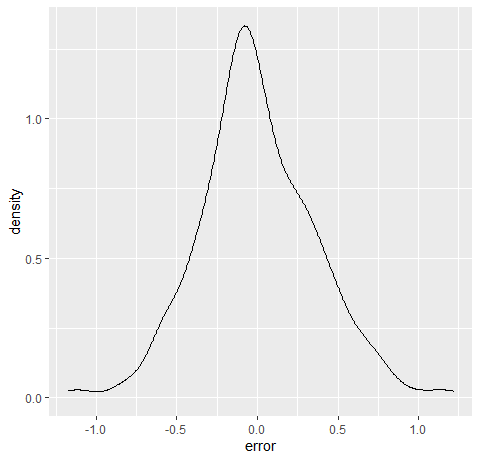
\includegraphics[width=.4\linewidth]{figures/errDist.png} }}
    \qquad
    \subfloat[\centering Q-Q Plot of Errors]{{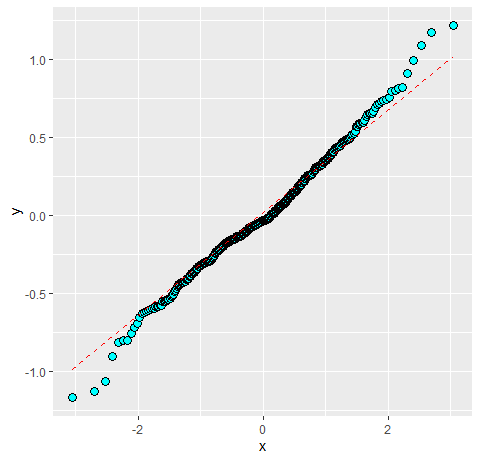
\includegraphics[width=.4\linewidth]{figures/errorqq.png} }}
    \caption{Error distribution with Q-Q plot}
    \label{errDistAndQQ}
\end{figure}

As we can see in this figure, there is a general bell curve, but not quite perfect as we have a bump between -0.5 and -0.75, as well as between 0.125 and 0.5. This 
non-normality is reflected in the Q-Q plot of the error. Measuring accuracy of the results is harder for these value prediction networks is harder than in classification 
problems. This is because we can't construct a prediction matrix. We don't expect the network to predict values down to the exact run, this would require a lot more 
data than is available, and a large amount of experimentation. One metric we can therefore use to see how accurate our model is, is to calculate 
the corrolation between the actual results and the predicted results. Using the inbuilt \textit{cor()} function, we obtain a corrolation value of 
$0.9382$. Given how close this is to 1, which would be perfect corrolation, it is fair to say that this method has done well to predict scores. \\

The issue that one may point out here is that this network has been trained on a full-over dataset, and then been tested on a full-over dataset. But the purpose of this 
investigation has been to look at the scenario in which a full game has been completed. So the method is currently ineffective at doing the task it set out to solve. For this reason,
we must come up with a way to 'fill in' the missing overs. The idea for this is to use Monte-Carlo simmulation. We discussed in \ref{exprr} how depending on the stage of the game,
the runrates can be drawn from one of three normal distributions. So for the overs that are missed, we can simply fill in the gaps by drawing a value from the distribution that the missing over falls 
into. 

\section{Interlude: Monte-Carlo Simmulation}
\label{mcsim}
Before simmulating cricket games to test our network on, we first find it necessary to delve into the mathematics of the methods used to for doing the simmulating. This is where
``Monte-Carlo'' simmulating comes in. \\
Let H be some random variable. At this stage, the distribution of H is irrelevant, but we note that $\mu = E(H)$. Formally, we have the following definition.

\begin{definition}
    Let $n \in \mathbb{N}$ and let $\{H_i \ | \ i =1,\ldots,n\}$ be i.i.d copies of H. The \textbf{Monte-Carlo Estimate} of $\mu$, is given as $\hat{\mu}=\frac{1}{n}\sum_{i=1}^n H_i$.  
\end{definition}

Recall the well-known \textit{Strong Law of Large Numbers}.

\begin{theorem}
    \label{slln}
    Let $n \in \mathbb{N}$, and let $H_1$,$H_2$,... be an i.i.d sample from a distribution with expectation $\mu$ and standard deviation $\sigma$, with $\mu, \ \sigma < \infty$.
    Then 
    $$ 
        P\left( \lim_{n \to \infty} \bar{H}_n = \mu \right) = 1
    $$
\end{theorem}

It follows from Theorem \ref{slln} that

\begin{align}
\lim_{n \to \infty} \hat{\mu} &= \lim_{n \to \infty} \frac{1}{n}\sum_{i=1}^nH_i \\
                              &= E(H) \\
                              &= \mu.
\end{align}

\section{Match Simulation}
With the theoretical framework for Monte-Carlo simmulation established, we can now look to build an algorithm for simmulating cricket matches. Based on our own work in Chapter 4, 
we begin by defining three random variables, $R_{\text{powerplay}} \sim N(\mu_{\text{powerplay}},\sigma_\text{powerplay})$, $R_{\text{middle}} \sim N(\mu_{\text{middle}},\sigma_{\text{middle}})$
and $R_{\text{final}} \sim N(\mu_{\text{final}},\sigma_{\text{final}})$.

The numerical values for these are given in the following table.

\begin{table}[h]
    \centering
    \begin{tabular}{c | c | c}
        Numerical Values & $\mu$ & $\sigma$ \\
        \hline
        $R_{powerplay}$ & 1.5298 & 0.4486 \\
        $R_{middle}$ & 1.6541 & 0.3355 \\
        $R_{final}$ & 3.1493 & 1.1349 
    \end{tabular}
    \caption{Numerical values of the parameters used for Monte-Carlo simmulation}
\end{table}

The code for doing this simmulation was not hard to write, and after a few small performance enhancements ran almost instantaneously. The code can be seen in figure \ref{mcecode}.

\begin{figure}[h] %MAKE SURE THESE ARE THE RIGHT LINES OF CODE!!
    \label{mcecode}
    \lstinputlisting[language=R, firstline=5,lastline=25]{../code/PyScripts/monteCarlo.py}
    \caption{Implementing a Monte-Carlo Simmulation fo Cricket Matches}
\end{figure}

It is best to think of n as a sort of fine-tuning parameter. If we have n too large, we would simply be simmulating the average cricket game, while have n too low and 
we are open to having an outlier. As for the other parameters, we have \textit{overs} being the number of overs in the game, and \textit{state} determines the over to start 
simmulating from. So if we want to simmulate the whole game, set $state=1$ and $overs=50$. The array \textit{runrates} just holds the data.\\

We then have the function \textit{MCE(n,state)}. The first line of this is a ``Ternary Operator'' to determine a parameter $t$. The job of $t$ is to be an index which obtains 
the correct parameters from the arrays in lines 2 and 3. This is then fed into the next line, uses the \textit{random.normalvariate()} function to populate an empty list with random 
values drawn fro the appropriate distribution of R. This is then averaged and returned by the function. Completing the main part of the Monte-Carlo method.
Finally, a while-loop runs through the overs needed and adds the estimation values to the \textit{runrates} array. \\

To give an idea of how the value of $n$ affects the resulting simmulation, we ran two simulations, using a small value $n=5$, and a larger one using $n=100$. 

\begin{figure}[h]
    \centering
    \subfloat[\centering $n=5$]{{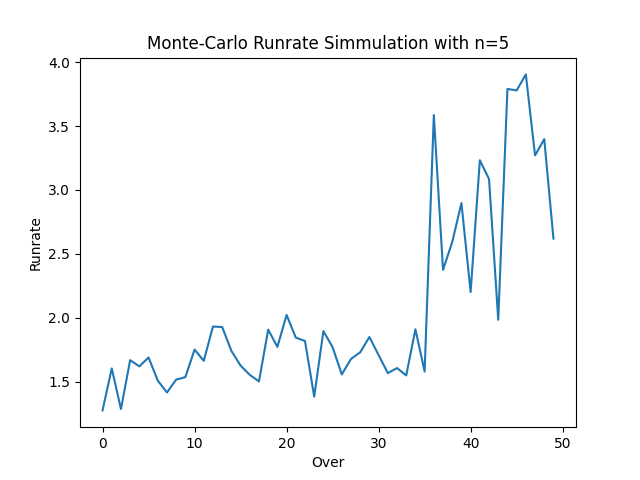
\includegraphics[width=.4\linewidth]{figures/mcen5.png} }}
    \qquad
    \subfloat[\centering $n=100$]{{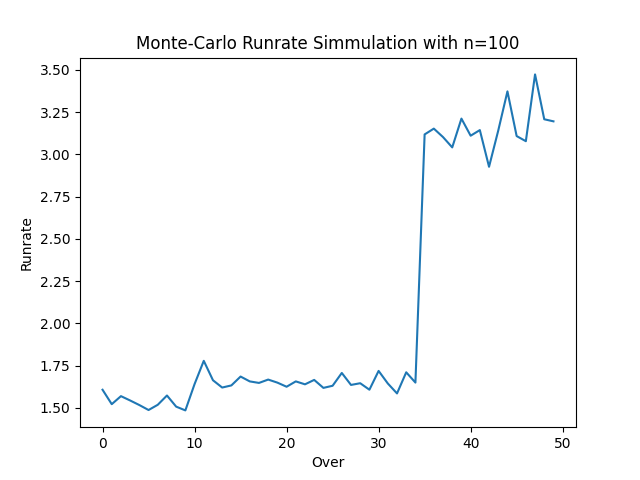
\includegraphics[width=.4\linewidth]{figures/mcen100.png} }}
    \caption{50-Over simmulation of $n=5$ and $n=100$}
    \label{MeanAndSDRR}
\end{figure}

If we compare these figues with (a) in Figure \ref{MeanAndSDRR}, we see that with large $n$, we have fallen victim to the ``Central-Limit Theorem'', and it looks as if the three 
sections of the game are unrelated. In the end, $n=20$ was the chosen value as it provided an appropriate middleground. \\

Testing if Monte-Carlo simmulation works was done in R by first cutting off each game in the original test set and random points, filling the rest in using the Monte-Carlo algorithm 
as previously described, and then feeding this into the neural network we built in the prior chapters. 

\begin{figure}[h]
    \centering
    \subfloat[\centering Error in Predictions from Monte-Carlo Simmulation]{{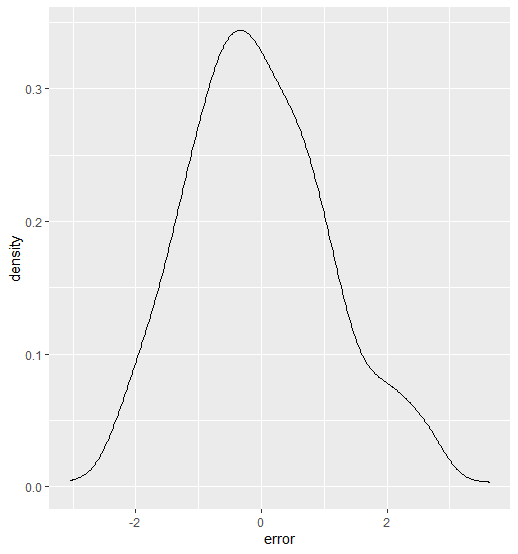
\includegraphics[width=.4\linewidth]{figures/monteCarloSimError.png} }}
    \qquad
    \subfloat[\centering Q-Q Plot of Monte-Carlo Prediction Errors]{{\includegraphics[width=.4\linewidth]{figures/monteCarloErrorQQ.png} }}
    \caption{Monte-Carlo Simmulation Error Density}
    \label{mcerror}
\end{figure}

Up until an error of around 2, we see this was more normally distributed than the original predictions. It is worth noting that this could be a side-effect of the fact that during the monte-carlo 
simmulation, all the games are being drawn directly from a normal distribution. To see definatively how the model compares to the neural network with full data, we take the corrolation of the actual results with those of the predicted values. 
We find that $\rho_{Network} = 0.9382$ and $\rho_{Monte-Carlo} = -0.0636$. So we see that when filling in the gaps with monte-carlo methods, the performance drops significantly. To further see this difference in performance, 
we calculate the difference of the monte-carlo method predictions and the original predictions, and take a boxplot.

\begin{figure}[h]
    \centering
    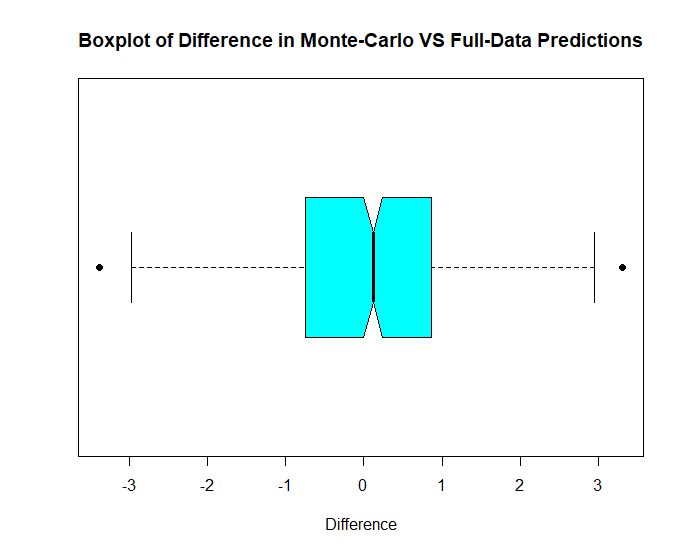
\includegraphics[scale=0.6]{figures/diffbox.png}
    \caption{Boxplot of prediction differences}
    \label{diffbox}
\end{figure}

We can see in Figure~\ref{diffbox}, that the difference is mostly centered around 0, which is promising, but the fact the corrolations are close to 0 means this is not a reliable method for predicting 
cricket scores. This is clearly an issue, because when it comes to resetting scores, the game obviously wont have a full 50 overs played, and so we need to fill in the gaps. We can then decrease the target score in proportion 
with the number of overs lost.

To put these results in more context, the data must be unscaled. The data was originally scaled using the base-R function \textit{scale()}. This applies the function

\[
    x_{\text{scaled}} = \frac{x_{\text{original}}-\mu}{\sigma}.    
\]

The parameters in the scaling can be re-obtained in R using the \textit{attr()} function. So implementing a function that 
performs unscaling on a new dataset is not too difficult, and can be achieved in afew lines of code. Note that the value of 51 has been hardcoded 
here as this is the column in which the runs scored are stored, but to make this more general, that value could be assigned dynamically.

\begin{figure}[h]
    \lstinputlisting[language=R, firstline=56,lastline=64]{../Code/Rscripts/monteCarlo.R}
    \caption{R function for unscaling data}
    \label{unscale}
\end{figure}

The function allows us to then see the actual predicted runs from both the complete neural network, and the neural network with 
gaps filled in via the Monte-Carlo method. Once this is done, for each game in the test set we plot the actual score, the score predicted by the full neural network and 
the score as predicted via the monte-carlo method. 

\begin{figure}[h]
    \label{fullPredDist}
    \centering
    \caption{Plot of predictions for all methods}
    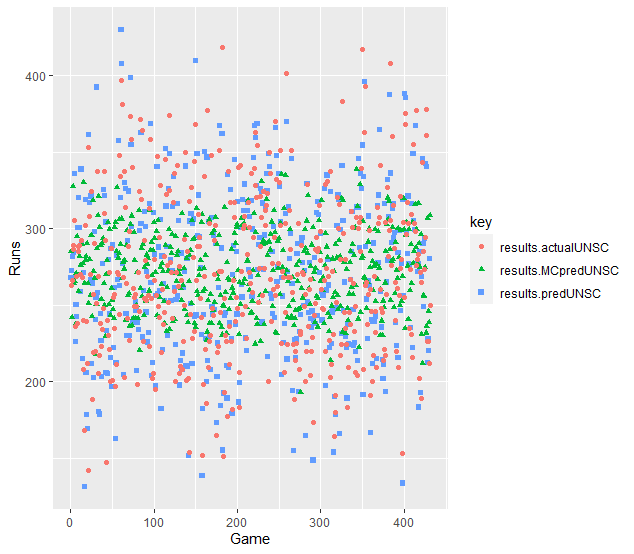
\includegraphics[scale=0.6]{figures/fullPredDist.png}
\end{figure}

This plot is naturally very busy, and it wont be used for detailed analysis of the accuracy, but what it does do well is give an overarching picture of the predictions. 
We can see that while the spread of red (actual scores) and blue (full network predictions) aren't too dissimilar, the spread of green points (monte-carlo predictions) is small and centered mainly 
around average game scores. This explains the poor performance of the model, it doesn't fair well with games that deviate far from the average. It is natural to ask how we can fix this. The one way that 
could lead to higher performance is to shrink the game into smaller chunks. Rather than looking at the three meta-stages of the game as we did originally, what about drawing from distributions of every 5 or 10 overs.

\section{Unseen DLS Game Data}
Since using Monte-Carlo methods didn't work too well, the next step is to look at seeing if something simpler will work. To do this, we take games that were decided through DLS, and 
feed them into the network to see how well it does. Rather than filling in the blanks of overs not played, we just set the runrate to 0 in these overs, and feed the resulting games into the neural network. 
We took 51 games which were decided by DLS, and looked at what the target set by DLS was. 

The results for this were actually better than for the monte carlo gap filling method. We achieved a corrolation in the results of 0.4983. Which is naturally lower than we would like, but a large improvement 
on the prior method. We can see in Figure~\ref{dlspreds} how the spread of points isn't in a narrow band as it was with monte carlo predictions. 

\begin{figure}[h]
    \label{dlspreds}
    \centering
    \caption{Network predictions for DLS games}
    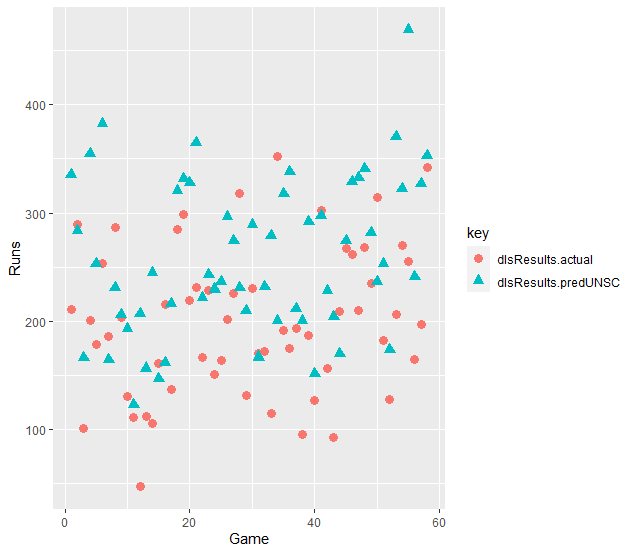
\includegraphics[scale=0.6]{figures/dlsPreds.png}
\end{figure}

We can also, as is standard practice, look at the errors of the predictions made by this model.

\begin{figure}[h]
    \label{dlsErrors}
    \centering
    \caption{DLS Prediction Errors}
    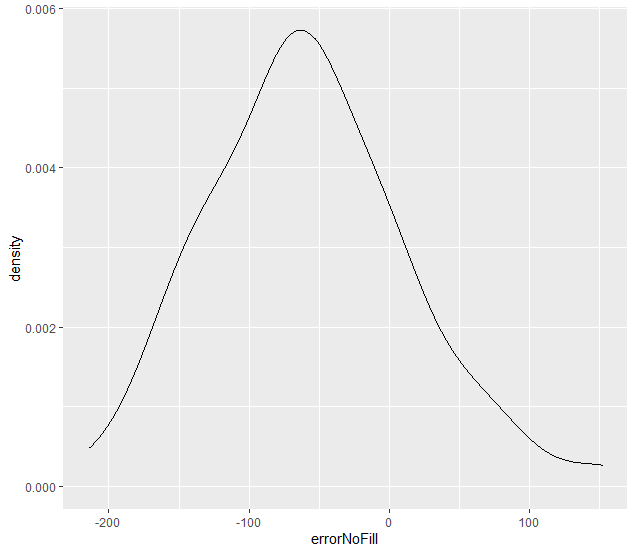
\includegraphics[scale=0.6]{figures/dlsErrorDist.png}
\end{figure}

These errors are follow a rough bell-curve shape, however we must remember that there aren't many datapoints here, so it may well be that with more datapoints, we would see more of a normal distribution. The downside however is 
that this curve is not centered around an error of 0, but around -58.22. This means that on average, the model sets teams a target of a much higher score. 

\section{England VS South Africa, 1992 World Cup}
In this section, we take the models that were produced in the prior chapter and apply them to the controversial game at the 1992 Australian Cricket World Cup. In the second semi-final,
played between England and South Africa at the Sydney Cricket Ground. England had not completed their 50 overs by 18:10pm, and so the number of overs was reduced to 45 overs. In South Africa's
innings, rain stopped play 5 balls into over 43. At this point in the game, South Africa were 231/6 with 13 balls left, chasing 253. The game was reduced to 43 overs, and using the \textit{most 
productive overs method}, South Africa were set a target of 252 off 43 overs, leading to the impossible requirement of 21 off 1 ball.\footnote{At the time, the electronic scoreboard at the ground,
and the TV coverage incorrectly displayed 22 to win off 1 ball.}

Note the afforementioned \textit{Most Productive Overs Method} is given by the equation:

\begin{equation}
    \text{Target in X overs} = \text{Runs scored by Team 1 in their highest-scoring X overs} + 1.
\end{equation}

A Duckworth-Lewis calculation was done retrospectively, and would have first set South Africa a target of 273 fron 45 overs, then 257 from the 43 overs.




\chapter{Conclusions and Future Work}

\epigraph{I'm completely cricketed out. If I never have to write another word about cricket again, I'll be a happy man.}{Joseph O'Neill}

\section{Conclusions}




\section{Discussion and Future Work}
Following on from what was mentioned in Section~\ref{mcsim}, rather than simply decreasing scores in proportion with the number of overs loft, 
it would be worth investigating decreasing the score depending on the fall of wicket distribution, as we looked at earlier in the paper. This could be 
done using Bayesian Techniques. \\

It's worth looking at expanding on the monte-carlo method; more specifically, breaking the game up into smaller stages to see how the accuracy of the model changes.

\bibliography{refs}{}
\bibliographystyle{plain}




\end{document}